\documentclass[showpacs,aps,floatfix,prb,reprint,superscriptaddress]{revtex4-1} 
%\documentclass[showpacs,floatfix,aps,prb,preprint,superscriptaddress]{revtex4-1}
%\documentclass[reprint,aps,groupedaddress]{revtex4-1}
\usepackage{xfrac}
\usepackage{amssymb}
\usepackage{braket}
\usepackage{graphicx}
%\usepackage{floatfix}
\usepackage{verbatim}
\usepackage{etoolbox}
\usepackage{amsfonts} %maths
\usepackage{amsmath} %maths
%\usepackage[fleqn]{amsmath} %maths
\usepackage[utf8]{inputenc} %useful to type directly diacritic characters
\usepackage{mathtools}
\usepackage{soul,xcolor,colortbl}
\usepackage{hyperref} \hypersetup{colorlinks=true,citecolor=blue,linkcolor=blue,urlcolor=blue} % HYPERLINKS
%\usepackage{widetext} %ELSEVIER

 \usepackage{ulem}
\usepackage{bm} %revtex4.1 for bold symbols
\usepackage{array}
\usepackage{color} % STEFANO


\begin{document}
\title{\Large Predicting intrinsic ductility in hexagonal close packed metals and alloys from elastic constants}
\author{Maarten de Jong, Axel van de Walle, Mark Asta}
\affiliation{Department of Materials Science and Engineering, University of California, Berkeley, 475 Hearst Memorial Mining Building, Berkeley, USA}


\date{\today}

\begin{abstract}
A solid's ideal strength corresponds to the stress at which the lattice itself becomes elastically unstable and hence, sets an upper bound on the mechanical strength that a material can have. The type of failure that occurs at the ideal strength can be related to the intrinsic ductility of the material. In this work, first principles-calculations are employed to show that all ideal (defect-free) hexagonal close packed metals fail in shear (intrinsically ductile behavior) rather than tension (intrinsically brittle behavior) when pulled in tension perpendicular to the basal plane, except Be, Mg, Ru, Os and Zn. In particular, among the metals that fail in shear, rhenium exhibits the highest shear modulus. These new results can be used to explain the observed ductile or brittle behavior among this important class of engineering materials. Also, a novel analytical model is proposed that predicts if hexagonal close packed metals and alloys fail in shear or tension based on just the second and third order elastic constants. For the transition metals in particular, filling of the $d$-bands is shown to govern what type of failure occurs under tension along the $c$-axis. In the spirit of $d$-band filling, we map out domains of the periodic table where ductile or brittle ideal failure occurs.  This can provide alloy designers with approximate alloy design-rules for which compositions lead to ductile hexagonal close packed alloys.
\end{abstract}

\maketitle

\section{Introduction}
A solid's ideal strength corresponds to the stress at which the lattice itself becomes elastically unstable and hence, sets an upper bound on the mechanical strength that a material can have. The ideal strength is of interest for another reason, namely because it sheds light on the deformation mechanisms and ductility in solids. At an atomistic level, the nucleation of a dislocation requires that the local shear stress on the slip plane is approximately equal to the ideal shear strength. On the other hand, crack initiation requires that the local normal stress, perpendicular to the cleavage plane is equal to or larger than the ideal tensile strength \cite{li2007ideal,clatterbuck2003ideal,kelly1986strong,wang2013estimate}. Upon loading an ideal solid to the ideal strength, different modes of failure may occur. When a material is loaded in tension perpendicular to the cleavage plane, it does not necessarily fail in a tensile mode in the loading direction, but may also fail in shear in a different orientation \cite{PhysRevLett.91.135501,PhysRevLett.112.115503,macmillan1983ideal,roundy2001ideal,wang2009elastic}. The type of failure that occurs first is of considerable interest as it is directly related to the instrinsic ductility of a solid. In particular, in the case of a shear instability, dislocation nucleation will be activated before crack formation, and the materials will be intrinsically ductile. It has been shown computationally in the literature that some well known highly ductile cubic metals such as vanadium (V) and niobium (Nb) indeed fail by shear rather than tension when pulled in uniaxial tension, whereas more brittle materials such as tungsten (W) and molybdenum (Mo) fail in shear \cite{PhysRevLett.112.115503}. First principles calculations of ideal strength and deformation behavior have been applied in the literature to study the intrinsic ductility of elemental metals as well as recently alloys \cite{PhysRevLett.82.2713,PhysRevB.87.214203,vsob1997theoretical,PhysRevB.58.6006}. It has also been shown that Mo-alloys can be made more intrinsically ductile by tuning the $d$ band filling to regions where a shear instability occurs before the onset of a tensile instability \cite{PhysRevLett.112.115503}.  \\

HCP metals and alloys constitute an important class of engineering materials, used for example in the aerospace and automotive industries. HCP transition metals often possess attractive properties such as high strength-to-weight ratio's, high stiffness and high melting temperatures. However these materials may exhibit low ductility due to the limited number of active slip systems. Hence, a lot of interest lies in strategies to optimize the ductility of HCP metals and alloys, for example by alloying. Despite the importance of hexagonal close packed (HCP) metals and alloys, the ideal strength, deformation behavior and intrinsic ductility of this class of materials have not been studied extensively in the literature. Although the ideal strengths of a few HCP-metals have been reported in the literature \cite{fu2012first}, no attempts at studying intrinsic ductility or ductility optimization have been made to the best of our knowledge. This is in stark contrast to the cubic metals, which have almost all undergone detailed investigations of their ideal strength and deformation behavior. Presumably, the case of HCP metals is more difficult due to their lower crystal symmetry and the corresponding richer variety of loading and deformation paths. \\

In this work we first consider the deformation behavior of the HCP-metals Be, Mg, Sc, Y, Ti, Zr, Hf, Tc, Re, Ru, Os, Co, Cd and Zn, when pulled perpendicular to the basal plane, which is a typical cleavage plane in HCP-metals and alloys \cite{yoo1981slip}. Based on the ideal deformation behavior, each of these HCP metals is characterized as intrinsically brittle (tensile elastic instability encountered first) or ductile (shear instability encountered first). We further study the ideal deformation behavior of HCP-based transition metal alloys and map out $d$-band filling domains where ductile vs brittle behavior can be expected. Ideal strength-calculations and finding elastic instabilities from Density Functional Theory (DFT) are rather computationally expensive. To mitigate this problem, in this work an analytical formalism is proposed to approximate the occurence of elastic instabilities from a knowledge of just the second and third order elastic constants of the solid. We find the results of the explicit DFT and the elasticity formalism to be in reasonable agreement across all HCP metals studied in this work. \\

The outline of this paper is as follows. We start by presenting the methodology, describing ideal strength and elastic instabilities in HCP metals, followed by a description of the calculation of higher order elastic constants. The details of our DFT-calculations are also presented. The results and discussion are then presented, followed by the conclusions.


\section{Methodology}
\subsection{Wallace-formalism and elastic instabilities in HCP-materials}
The elastic stability of a solid under zero stress is governed by the eigenvalues of its elastic tensor. It is well-known that all 6 eigenvalues should be larger than zero for the solid to be elastically stable. For a solid under an applied stress however, elastic stability is formulated in terms of the Wallace-tensor, which is defined in Eq. \ref{eqn:Wallace1}. In this equation, $C_{ijkl}'$ represents the elastic constants in the deformed configuration \cite{wallace1998thermodynamics,ray1988elastic,wang1993crystal} and $\sigma$ represents the stress tensor acting on the solid. Finally, $\delta$ represents the Kronecker-delta. The eigenvalues of the symmetrized Wallace-tensor govern the elastic stability of a solid under stress.

\begin{equation}
\label{eqn:Wallace1}
B_{ijkl} = C_{ijkl}' + \frac{1}{2} \left(\sigma_{il} \delta_{jk} + \sigma_{jl} \delta_{ik} + \sigma_{ik} \delta_{jl} + \sigma_{jk} \delta_{il} - 2\sigma_{ij} \delta_{kl} \right)
\end{equation}

Eq. \ref{eqn:Wallace1} holds true for solids of any crystal symmetry. It can be simplified considerably by assuming a given crystal structure and loading direction. First, for HCP metals and alloys the elastic tensor in Voigt notation (at zero external stress) reduces to the form shown in Eq. \ref{eqn:Cijref}. It is also important to note that as an HCP-material is pulled along $c$ and relaxed in the basal plane, the $c/a$-ratio changes but the hexagonal symmetry is maintained and hence, the elastic tensor symmetry does not change. Second, for an HCP-material under uniaxial tension along the $c$-axis, the only non-zero stress component is $\sigma_{33}$ and we can write the stress tensor simply as in Eq. \ref{eqn:solidstress1}. For this specific loading situation, the expression for the symmetrized Wallace-tensor takes a particularly simple form, see Eq. \ref{eqn:Wallace2}.

\begin{equation} 
\label{eqn:Cijref} 
C_{ij} 
=
\left[
\begin{array}{cccccc}
C_{11} & C_{12} & C_{13} & 0 & 0 & 0 \\
C_{12} & C_{11} & C_{13} & 0 & 0 & 0 \\
C_{13} & C_{13} & C_{33} & 0 & 0 & 0 \\
0 & 0 & 0 & C_{44} & 0 & 0 \\
0 & 0 & 0 & 0 & C_{44} & 0 \\
0 & 0 & 0 & 0 & 0 & \frac{1}{2} \left(C_{11}-C_{12} \right)\\
\end{array}
\right]
\end{equation}

\begin{equation}
\label{eqn:solidstress1}
\mathbf{\sigma} =  \begin{bmatrix}
       0 & 0 & 0           \\[0.3em]
       0 & 0           & 0 \\[0.3em]
       0           & 0 & \sigma_{33}
     \end{bmatrix}
\end{equation}

\begin{widetext}
\begin{equation}
\label{eqn:Wallace2}
B_{ijkl} = \begin{bmatrix}
C_{11}' & C_{12}' & C_{13}' + \frac{\sigma_{33}}{2} & 0  & 0 & 0  \\[0.20em]
C_{12}' & C_{11}' & C_{13}' + \frac{\sigma_{33}}{2} & 0  & 0 & 0   \\[0.20em]
C_{13}' + \frac{\sigma_{33}}{2} & C_{13}' + \frac{\sigma_{33}}{2}  & C_{33}'-\sigma_{33}  & 0  & 0 & 0  \\[0.20em]
0  & 0 & 0 & C_{44}'-\frac{\sigma_{33}}{2} & 0 & 0 \\[0.20em]
0  & 0 & 0 & 0 & C_{44}'-\frac{\sigma_{33}}{2} & 0  \\[0.20em]
0  & 0 & 0 & 0 & 0 & \frac{C_{11}'-C_{12}'}{2}  \\[0.20em]
\end{bmatrix}
\end{equation}
\end{widetext}

The eigenvalues of Eq. \ref{eqn:Wallace2} determine the elastic stability of an HCP-material under uniaxial tension along the $c$-axis. The terms $C_{ij}'$ appearing in Eq. \ref{eqn:Wallace2} are the elastic constants in the deformed configuration. The Wallace-tensor $B_{ijkl}$ in Eq. \ref{eqn:Wallace2} has 5 distinct eigenvalues, 3 of which involve the stress $\sigma_{33}$ explicitly. The two relevant eigenvalues for this work are given in Eqs. \ref{eqn:Wallace3} and \ref{eqn:Wallace4}.

\begin{equation}
\label{eqn:Wallace3} 
\lambda_{1} = C_{44}' - \frac{\sigma_{33}}{2} 
\end{equation}


%\begin{multline}
\begin{widetext}
\begin{multline}
%\begin{equation}
\label{eqn:Wallace4}
\lambda_{2} =  \frac{C_{11}' + C_{12}' + C_{33}' - \sigma_{33}}{2} - \\ \frac{\sqrt{(C_{11}'^2 + 2C_{11}'C_{12}' - 2C_{11}'C_{33}' + 2C_{11}'\sigma_{33} +  C_{12}'^2 - 2C_{12}'C_{33}' + 2C_{12}'\sigma_{33} + 8C_{13}'^2 + 8C_{13}'\sigma_{33} + C_{33}'^2 - 2C_{33}'\sigma_{33} + 3\sigma_{33}^2)}}{2}
%\end{equation}
\end{multline}
\end{widetext}
%\end{multline}

The eigenvalue $\lambda_{1}$ in Eq. \ref{eqn:Wallace3} is associated with the eigenvector $v_{1} = \left(0, 0, 0, 1, 1, 0\right)$, which represents a shear instability. The eigenvalue $\lambda_{2}$ on the other hand, is associated with the eigenvector $v_{1} = \left(0, 0, 1, 0, 0, 0\right)$ which represents a tensile instability along the direction of loading (the $c$-axis). Upon loading the crystal along the $c$-axis, if the eigenvalue $\lambda_{1}$ attains negative values before the eigenvalue $\lambda_{2}$, the crystal fails in shear. If not, the crystal fails in tension. As mentioned in the introduction of this paper, failure in tension or shear of the ideal crystal is relevant to the mechanical properties of true materials.  \\

Eqs. \ref{eqn:Wallace3} and \ref{eqn:Wallace4} contain the elastic constants of the crystal in its deformed state. These can be obtained in principle by calculating the elastic tensor from DFT for each structure along the strain path. However, this is a computationally expensive procedure and it does not lead to a clear physical understanding of the underlying physics leading to the elastic instabilities. Instead, the elastic constants in the deformed configuration, $C_{ij}'$, can also be approximated from the third order elastic constants (TOEC's) and the standard second order elastic constants at zero stress (SOEC's). For small strains around a zero strain-state, the elastic constants can be approximated to be constant as a function of strain, i.e. $C_{ij} = C_{ij}'$. However, elastic instabilities typically occur for strains of over 10 \% (with some exceptions, such as Nb) and hence, the elastic constants in the strained configuration will deviate significantly from those in the zero strain-configuration, i.e. $C_{ij} \neq C_{ij}'$. The TOEC's dictate how the elastic constants $C_{ij}'$ evolve as a function of the imposed strain. Let $\xi = \eta_{33}$ represent the (imposed) tensile strain along the $c$-axis of an HCP-materials and let $\eta = \eta_{11} = \eta_{22}$ be the resulting strain in the basal plane (usually contraction in accordance with a positive Poisson's ratio). For that particular strain state, the expressions for $C_{11}'$, $C_{12}'$, $C_{13}'$, $C_{33}'$ and $C_{44}'$ are given in Eqs. \ref{eqn:Cprime} \cite{rao1969third,rao1974anderson}, where the terms $C_{ijkl}$ denote the 10 independent TOEC's for the HCP-materials studied in this work \cite{hearmon1953third,rose1968higher,fumi1951third,fumi1952third}. 

\begin{widetext}
\begin{subequations}
\label{eqn:Cprime} 
\begin{align}
        C_{11}' &=C_{11} + \eta \left(4 C_{11} + 2C_{12} + C_{111} + C_{112}\right) + \xi \left(-C_{11} + 2C_{13} + C_{113}\right),\\
        C_{12}' &=C_{12} + \eta \left(C_{111} + 2C_{112} - C_{222} + 2C_{12}\right) + \xi \left(-C_{12} + C_{123}\right),\\
				C_{13}' &=C_{13} + \eta \left(C_{113} + C_{123} \right) + \xi \left(C_{13} + C_{133}\right),\\
				C_{33}' &=C_{33} + \eta \left(4C_{13} - 2C_{33} + 2C_{133} \right) + \xi \left(5C_{33} + C_{333}\right),\\
				C_{44}' &=C_{44} + \eta \left(\frac{1}{2} C_{11} + \frac{1}{2} C_{12} + C_{13} + C_{144} + C_{155} \right) + \xi \left(\frac{1}{2} C_{13} + \frac{1}{2} C_{33} + C_{44} + C_{344}\right)
\end{align}
\end{subequations}
\end{widetext}

We now proceed by eliminating $\eta$ from Eqs. \ref{eqn:Cprime} by expressing it in term of $\xi$. The imposed strain along $c$, $\xi$, and the resulting strain in the basal plane, $\eta$, are related by just the Poisson's ratio for small strains. For large strains $\xi$ however, the TOEC's have to be invoked to calculate $\eta$. To this end, we first introduce some additional notation. \\

Consider the mapping between the reference and current configuration of a continuum solid. In the reference configuration, a particle occupies a point $\bm{p}$ with spatial coordinates $\bm{X} = X_{1}\bm{e}_{1} +  X_{2}\bm{e}_{2} + X_{3}\bm{e}_{3}$, where ${e}_{1}, {e}_{2}, {e}_{3}$ is a Cartesian reference triad and $X_{1}, X_{2}, X_{3}$ are the reference coordinates. Upon deformation of the body, the point originally at $\bm{X}$ is translated by the displacement vector $\bm{u} \left(X_{1}, X_{2}, X_{3} \right)$ to its final coordinates $\bm{x} \left(X_{1}, X_{2}, X_{3} \right)$, see Eq. \ref{eqn:displ1} .
\begin{equation}
\label{eqn:displ1} 
\bm{x} \left(X_{1}, X_{2}, X_{3} \right) = \bm{u} \left(X_{1}, X_{2}, X_{3} \right) + \bm{X} \left(X_{1}, X_{2}, X_{3} \right)
\end{equation}

Based on this description, a deformation gradient is formulated as in Eq. \ref{eqn:defgrad1}. The Green-Lagrange strain tensor $\bm{\eta}$ then follows from $\bm{F}$ as shown in Eq. \ref{eqn:GL1}, where $\bm{I}$ denotes the identity matrix.
\begin{equation}
\label{eqn:defgrad1} 
\bm{F} = \frac{\partial x_{i}}{ \partial X_{j}}
\end{equation}

\begin{equation}
\label{eqn:GL1} 
\bm{\eta} = \frac{1}{2} \left(\bm{F}^{T} \bm{F} - \bm{I} \right)
\end{equation}

With the notation now established, the strain energy density can be expanded in terms of the SOEC's, TOEC's and the Green-Lagrange strain  as in Eq. \ref{eqn:expansion1}, where $\rho_{0}$ represents the mass density in the undeformed state and the terms $\eta_{i}$ represent the components of the tensor defined in Eq. \ref{eqn:GL1}. The symmetry of the SOEC's and TOEC's will be applied in the expansions, which simplifies the resulting expressions considerably.

\begin{equation}
\label{eqn:expansion1} 
\rho_{0} E \left(\bm{\eta}\right) = \frac{1}{2!} \sum_{i,j=1}^{6} C_{ij} \eta_{i} \eta_{j} + \frac{1}{3!} \sum_{i,j,k=1}^{6} C_{ijk} \eta_{i} \eta_{j} \eta_{k} + \ldots
\end{equation}

Consider an imposed strain $\xi$ along the $c$-axis of an HCP-metal, initially keeping all other dimensions fixed to the zero strain-state. Consider first the expansion of Eq. \ref{eqn:expansion1}, retaining only terms up to and including the SOEC's (hence, ignoring the TOEC's for now). This gives the energy-expression in Eq. \ref{eqn:expansion3}, in which the symmetry of the SOEC's has been applied. To obtain the equilibrium strain in the basal plane due to the application of $\xi$, we perform strain energy-minimization and set $\bar{\eta} = \eta = \eta_{1} = \eta_{2}$, $\eta_{3} = \xi$ and $\eta_{4} = \eta_{5} = \eta_{6} = 0$ in Eq. \ref{eqn:expansion3} and solve $\frac{\partial \left(\rho_{0} E\right)}{\partial \eta}|_{\xi} = 0$. We find the equilibrium strain $\eta = \bar{\eta}$, given in Eq. \ref{eqn:eqstr1}, where the minus-sign signifies the Poisson-contraction in the basal plane.

\begin{multline}
\label{eqn:expansion3} 
\rho_{0} E \left(\bm{\eta}\right) = C_{11}\frac{\eta_{1}^2}{2} + C_{11}\frac{\eta_{2}^2}{2} +  C_{33}\frac{\xi^2}{2} + C_{44}\frac{\eta_{4}^2}{2} + C_{44}\frac{\eta_{5}^2}{2} + \\  \frac{1}{2} \left(C_{11}-C_{12}\right)\frac{\eta_{6}^2}{2} + C_{12}\eta_{1}\eta_{2} + C_{13}\eta_{1}\xi + C_{13}\eta_{2}\xi
\end{multline}

\begin{equation}
\label{eqn:eqstr1} 
\eta = \bar{\eta} = -\frac{\xi C_{13}}{C_{11} + C_{12}}
\end{equation}

For large strains, the expansion in Eq. \ref{eqn:expansion3} is not sufficient and instead, TOEC's have to be included as well. The expansion of the strain energy up to the third order in strain is given in Eq. \ref{eqn:expansion2}, in which the terms $P$ are given in Eq. \ref{eqn:expansion2detailed}. Note that in Eq. \ref{eqn:expansion2}, the symmetry of the SOEC's and TOEC's has been incorporated to simplify the resulting expression. 

\begin{multline}
\label{eqn:expansion2} 
\rho_{0} E \left(\bm{\eta}\right) = C_{11} P_{1} +  C_{12} P_{2} + C_{13} P_{3} + C_{33} P_{4} + \\ C_{44} P_{5} + C_{111} P_{6} + C_{222} P_{7} + C_{333} P_{8} + \\ C_{133} P_{9} +  C_{113} P_{10} + C_{112} P_{11} + C_{123} P_{12} + \\ C_{144} P_{13} + C_{155} P_{14} + C_{344} P_{15}
\end{multline}


\begin{subequations}
\label{eqn:expansion2detailed} 
\begin{align}
        P_{1} &=\frac{\eta_{1}^2}{2}  + \frac{\eta_{2}^2}{2} + \frac{\eta_{6}^2}{4} ,\\
        P_{2} &=-\frac{\eta_{6}^2}{4} + \eta_{1}\eta_{2} ,\\
				P_{3} &=\eta_{1}\eta_{3} + \eta_{2}\eta_{3} , \\
				P_{4} &=\frac{\eta_{3}^2}{4} , \\
				P_{5} &=\frac{\eta_{4}^2}{2} + \frac{\eta_{5}^2}{2} , \\
				P_{6} &=\frac{\eta_{1}^3}{6} + \frac{\eta_{1}\eta_{2}^2}{2} - \frac{\eta_{1}\eta_{6}^2}{4} + \frac{\eta_{2}\eta_{6}^2}{4} , \\
				P_{7} &=\frac{\eta_{2}^3}{6} - \frac{\eta_{1}\eta_{2}^2}{2} - \frac{\eta_{2}\eta_{6}^2}{8} + 3\frac{\eta_{1}\eta_{6}^2}{8} , \\
				P_{8} &=\frac{\eta_{3}^3}{6} , \\
				P_{9} &=\frac{\eta_{1}\eta_{3}^2}{2} + \frac{\eta_{2}\eta_{3}^2}{2} , \\
				P_{10} &=\frac{\eta_{3}\eta_{1}^2}{2} + \frac{\eta_{3}\eta_{2}^2}{2} + \frac{\eta_{3}\eta_{6}^2}{4} , \\
				P_{11} &=\frac{\eta_{1}^2\eta_{2}}{2} +  \frac{\eta_{1}\eta_{2}^2}{2} - \frac{\eta_{6}^2\eta_{1}}{8} - \frac{\eta_{6}^2\eta_{2}}{8} , \\
				P_{12} &=\eta_{1}\eta_{2}\eta_{3} - \frac{\eta_{3}\eta_{6}^2}{4} , \\
				P_{13} &=\frac{\eta_{1}\eta_{4}^2}{2} + \frac{\eta_{2}\eta_{5}^2}{2} - \frac{\eta_{4}\eta_{5}\eta_{6}}{2} , \\
				P_{14} &=\frac{\eta_{2}\eta_{4}^2}{2} + \frac{\eta_{1}\eta_{5}^2}{2} + \frac{\eta_{4}\eta_{5}\eta_{6}}{2} , \\
				P_{15} &=\frac{\eta_{3}\eta_{4}^2}{2} + \frac{\eta_{3}\eta_{5}^2}{2} 
\end{align}
\end{subequations}

Given an applied $\xi$, we can again find an analytical expression for the Poisson contraction $\eta = \bar{\eta}$ in terms of $\xi$ and the SOEC's and TOEC's. The resulting equation that has to be solved is shown in Eq. \ref{eqn:minexpression1}. Solving Eq. \ref{eqn:minexpression1} in terms of $\eta = \bar{\eta} = \eta_{1} = \eta_{2}$ gives the equilibrium strain in the basal plane. This expression for $\bar{\eta}$ including the TOEC's is lengthy and is not presented here.

\begin{widetext}
\begin{equation}
\label{eqn:minexpression1}
\frac{\partial \left(\rho_{0} E\right)}{\partial \eta} |_{\eta_{1}=\eta_{2}, \eta_{4,5,6}=0} = \eta_{1}^{2} \left(2C_{111} + 3C_{112} - C_{222} \right) + \eta_{1} \left(C_{11} + 2C_{12} + 2C_{113} \xi + 2C_{123} \xi \right) + \xi^{2} C_{133} + 2\xi C_{13} = 0
\end{equation}
\end{widetext} 

With the theory developed above, a closed-form expression for predicting when elastic instabilities occur in HCP-materials in nearby. Upon applying $\xi$, the basal plane contracts by a strain $\bar{\eta} = \eta = \eta(\xi)$, which follows from Eq. \ref{eqn:minexpression1}. The expression for $\eta = \bar{\eta}$ can be substituted into Eqs. \ref{eqn:Cprime}, which eliminates $\eta$ and leaves $\xi$ as the only (control) variable. Subsequently, the expressions for $C_{ij}'$ can be substituted into Eqs. \ref{eqn:Wallace3} and \ref{eqn:Wallace4}. \\

To obtain the final closed-form expressions, we express the stress $\sigma_{33}$ in terms of the strain state, SOEC's and TOEC's. We first derive an expression for the true stress component $\sigma_{33}$. Eq. \ref{eqn:stressexpansion1} expresses the Lagrangian stress tensor in terms of the strain energy and Lagrangian strain tensor \cite{lopuszynski2007ab}. Eq. \ref{eqn:stressexpansion1} is employed to calculate the Lagrangian stress $t_{33}$, under a combined loading condition of $\eta_{1}=\eta_{2}=\bar{\eta}$ and $\eta_{3}=\xi$ simultaneously. The result is shown in Eq. \ref{eqn:t33eq1}. From Eq. \ref{eqn:stressconversion1}, we have that $\bm{\sigma} = \frac{1}{\text{det} \left(\bm{F}\right)} \bm{F} \bm{t} \bm{F}^{T}$. This expression can be expanded, with the result given in Eq. \ref{eqn:t33eq2}, where $t_{33}$ is given in Eq. \ref{eqn:t33eq1}. 


\begin{equation}
\label{eqn:stressexpansion1} 
t_{ij} = \rho_{0} \frac{\partial E}{\eta_{ij}}
\end{equation}

\begin{multline}
\label{eqn:t33eq1} 
t_{33} |_{\eta_{4,5,6} = 0} = \eta_{1}^{2} \left(C_{113} + C_{123} \right) + \eta_{1} \left(2C_{13} + 2C_{133}\eta_{3} \right) + \\ \frac{1}{2} C_{333} \eta_{3}^{2} + C_{33} \eta_{3}
\end{multline}

\begin{equation}
\label{eqn:stressconversion1} 
t_{ij} = \text{det} \left(\bm{F}\right) \bm{F}^{-1} \bm{\sigma} \left(\bm{F}^{T}\right)^{-1}
\end{equation}


\begin{equation}
\label{eqn:t33eq2} 
\sigma_{33}  = \frac{\sqrt{2 \xi + 1}}{\sqrt{2 \bar{\eta} + 1}}t_{33}
\end{equation}

An equation can now be set-up to determine for which strain $\xi$, a shear instability will first occur. Starting from Eq. \ref{eqn:Wallace3}, we substitute the expression for $C_{44}'$ from Eq. \ref{eqn:Cprime}. In this, $\eta_{3} = \xi$ is the control variable and $\eta = \eta_{1} = \eta_{2} = \bar{\eta}$ is the resulting contraction in the basal plane of the material, which can be analytically calculated from Eq. \ref{eqn:minexpression1}. Similarly, $\sigma_{33}$ follows from Eq. \ref{eqn:t33eq2}, with $t_{33}$ given in Eq. \ref{eqn:t33eq1}. Similarly, the strain at which a tensile elastic instability occurs can be derived by considering the eigenvalue in Eq. \ref{eqn:Wallace4} and substituting the expressions for $C_{ij}'$ and $\sigma_{33}$. The strain along $c$ at which an elastic instability (either shear or tensile) first occurs is indicated by $\bar{\xi}$ hereafter. \\

In summary, the above formalism allows us to estimate for which uniaxial stress state along the $c$-axis, elastic shear and tensile instabilites occur in hexagonal close packed metals and alloys. Of particular interest is whether the shear instability occurs before or after the tensile instability. In the former case the material is deemed intinsically ductile whereas in the latter case, it is deemed intrinsically brittle. The only input required for this formalism are the second and third order elastic constants. In the next section, it is explored how the TOEC's can be calculated for HCP-materials.


\subsection{Calculation of second and third-order elastic constants}
The previous section has laid out a methodology to study elastic instabilities in HCP-materials from the perspective of SOEC's and TOEC's. In this section, it is shown how these quantities can be calculated in a robust manner. Eq. \ref{eqn:stressexpansion1} expresses the stress tensor in terms of the energy and Lagrangian strain tensor. By applying a set of carefully constructed deformations to a cell, all 10 independent TOEC's can be extracted by fitting the stress components, as calculated from DFT, to the applied strains. The pertinent expressions are shown in Eqs. \ref{eqn:s1}-\ref{eqn:s12}, in which the following Voigt-notation is employed: $11 \mapsto 1$, $22 \mapsto 2$, $33 \mapsto 3$, $23 \mapsto 4$, $13 \mapsto 5$, $12 \mapsto 6$.

\begin{equation}
\label{eqn:s1} 
t_{1} \left(\eta_{1}\right) = \rho_{0} \frac{\partial E}{\partial \eta_{1}} = \frac{C_{111}\eta_{1}^2}{2} + C_{11}\eta_{1}
\end{equation}

\begin{equation}
\label{eqn:s2} 
t_{2} \left(\eta_{2}\right) = \rho_{0} \frac{\partial E}{\partial \eta_{2}} = \frac{C_{222}\eta_{2}^2}{2} + C_{11}\eta_{2}
\end{equation}

\begin{equation}
\label{eqn:s3} 
t_{3} \left(\eta_{3}\right) = \rho_{0} \frac{\partial E}{\partial \eta_{3}} = \frac{C_{333}\eta_{3}^2}{2} + C_{33}\eta_{3}
\end{equation}

\begin{equation}
\label{eqn:s4} 
t_{3} \left(\eta_{1}\right) = \rho_{0} \frac{\partial E}{\partial \eta_{3}} = \frac{C_{113}\eta_{1}^2}{2} + C_{13}\eta_{1}
\end{equation}

\begin{equation}
\label{eqn:s5} 
t_{1} \left(\eta_{3}\right) = \rho_{0} \frac{\partial E}{\partial \eta_{1}} = \frac{C_{133}\eta_{3}^2}{2} + C_{13}\eta_{3}
\end{equation}

\begin{equation}
\label{eqn:s6} 
t_{2} \left(\eta_{1}\right) = \rho_{0} \frac{\partial E}{\partial \eta_{2}} = \frac{C_{112}\eta_{1}^2}{2} + C_{12}\eta_{1}
\end{equation}

\begin{equation}
\label{eqn:s7} 
t_{4} \left(\eta_{4}\right) = \rho_{0} \frac{\partial E}{\partial \eta_{4}} = C_{44}\eta_{4}
\end{equation}

\begin{equation}
\label{eqn:s8} 
t_{3} \left(\eta_{3}, \eta_{5}\right) = \frac{C_{333}\eta_{3}^2}{2} + C_{33}\eta_{3} + \frac{C_{344}\eta_{5}^2}{2}
\end{equation}

\begin{equation}
\label{eqn:s9} 
t_{5} \left(\eta_{3}, \eta_{5}\right) = C_{44}\eta_{5} + C_{344}\eta_{3}\eta_{5}
\end{equation}

%\begin{equation}
%\label{eqn:s9} 
%t_{3} \left(\eta_{3}, \eta_{5}\right) = \frac{C_{333}\eta_{3}^2}{2} + C_{33}\eta_{3} + \frac{C_{344}\eta_{5}^2}{2}
%\end{equation}

\begin{equation}
\label{eqn:s10} 
t_{3} \left(\eta_{1}, \eta_{2}\right) = \frac{C_{113}\eta_{1}^2}{2} + C_{123}\eta_{1}\eta_{2} + C_{13}\eta_{1} +  \frac{C_{113}\eta_{2}^2}{2} + C_{13}\eta_{2}
\end{equation}


\begin{equation}
\label{eqn:s11} 
t_{4} \left(\eta_{1}, \eta_{4}\right) = C_{44}\eta_{4} + C_{144}\eta_{1}\eta_{4}
\end{equation}

\begin{equation}
\label{eqn:s12} 
t_{5} \left(\eta_{1}, \eta_{5}\right) = C_{44}\eta_{5} + C_{155}\eta_{1}\eta_{5}
\end{equation}

For each of the strain modes described in Eqs. \ref{eqn:s1}-\ref{eqn:s12}, strains are applied varying from -6 \% to + 20\%, in steps of 0.5 \%. Note that this strain range is considerably larger than what is commonly used for the calculation of the SOEC's, which typically varies from -2 \% to +2 \% strain. The TOEC's give rise to a nonlinear stress-strain behavior and this effect only becomes apparent at relatively large strains (larger than approximately 10 \% for the materials studied in this work), hence the extended strain range. \\

Eqs. \ref{eqn:s1}-\ref{eqn:s12} give rise to an overdetermined system that is solved for the 5 independent SOEC's and 10 independent TOEC's. A pseudo-inverse is employed to this end, calculated from a singular value decomposition. The values of the calculated TOEC's are found in this work to be rather sensitive to the precise strain range that is employed in the fitting, which has been observed also in the literature \cite{wang2009ab,lopuszynski2007ab,wang2012nonlinear}. For the HCP-metals and alloys studied in this work, the TOEC's converge to a plateau when approximately 11-16 \% maximum strain is used in the fit. Using smaller or larger maximum strains than those corresponding to the plateau can lead to TOEC's differing by up to a factor 5 for the systems studied in this work. For maximum strains within the plateau-region, TOEC's are generally converged to within 25 \% in this work. Consistent with other work in the literature, the location of this plateau dictates which precise strain range is used in the fitting \cite{wang2009ab,wang2012nonlinear}.



\subsection{DFT-calculations}
With the exception of the Virtual Crystal Approximation (VCA) results, all calculations were performed using the Vienna Ab Initio Simulation Package (VASP) \cite{PhysRevB.54.11169,PhysRevB.47.558}. The VASP calculations made use of the exchange-correlation energy as approximated by the Perdew-Burke-Ernzerhof generalized gradient functional (PBE-GGA) \cite{PhysRevLett.77.3865}.

All of these calculations made use of the projector augmented wave (PAW) method \cite{PhysRevB.50.17953,PhysRevB.59.1758}.  An energy cutoff for the plane waves of 700 eV was used, and smearing of the electronic occupancies was performed using the Methfessel-Paxton scheme \cite{PhysRevB.40.3616}, with a broadening of 0.05 eV.  Integrations in the Brillouin zone were carried out using Monkhorst-Pack $k$-point sampling \cite{PhysRevB.13.5188} with a density chosen such that the number of $k$-points in the first Brillouin zone times the number of atoms in the cell equals approximately 25,000. The employed PAW potentials for Sc, Ti, Y, Zr and Hf include $s$, $p$ and $d$-states as valence. For the other elements, only $s$ and $d$-states are used as valence. \\

For the purpose of investigating the origins of alloying effects on ideal deformation behavior, we also employed calculations based on the VCA  method. The VCA calculations were performed using the Quantum Espresso software \cite{giannozzi2009quantum}, employing norm-conserving Troullier-Martin pseudopotentials \cite{troullier1991efficient,romaner2010effect}. Use was made of the generalized gradient approximation, based on the Perdew-Burke-Ernzerhof exchange-correlation functional \cite{PhysRevLett.77.3865}. The pseudopotentials were generated using the fhi98PP code with intermediate nuclear charges \cite{fuchs1999ab}. 



\section{Results and Discussion}
In this section, results for most HCP transition metals and Mg and Be are shown. Lattice stabilities are calculated as a function of $c$-strain and the failure modes are studied. This allows for a division of the HCP-metals into two classes: those that are intrinsically ductile or brittle. Further, the effect of $d$-band filling is studied on the failure modes. This leads to a general overview of which classes of HCP-based alloys are intrinsically ductile and which are intrinsically brittle.

\subsection{Elastic instabilities in HCP materials: DFT and analytical model}
The Wallace-tensor (see Eq. \ref{eqn:Wallace2}) can be approximated from the above formalism by means of the SOEC's and TOEC's. However, in principle, it can be calculated explicitly from DFT for each strain along the $c$-deformation path. This direct DFT-approach is expensive since for every strain along the $c$-axis, it first requires a structural relaxation of the $a$ and $b$ lattice vectors and the atomic coordinates. Further, a calculation of the elastic constants in the deformed configuration, $C_{ijkl}'$, is required for each strained structure, which further increases the computational cost. Presumably, this direct DFT-approach to calculate the Wallace tensor and lattice instabilties is more accurate than the formalism based on the SOEC's and TOEC's, since it does not require the evaluation of the TOEC's and hence mitigates some of its associated inaccuracies and limitations. In this section, we calculate at which $c$-strain lattice instabilities occur in all HCP transition metals and Mg and Be. \\

The results are shown in Table \ref{tab:overview_elastic1}. Clearly, the analytical model predicts the ideal failure mode (either shear or tensile failure) correctly for 12 transition metals (Zn and Cd included in the definition of transition metals) and the 2 non-transition metals Be and Mg. Further, the critical $c$-strain ($\bar{\xi}$) at which an elastic instability first occurs is predicted to within an accuracy of approximately 4 \% strain. The differences in $\bar{\xi}$ calculated directly DFT and from the analytical model can be attributed to mainly 2 factors. First of all, the calculation of TOEC's from DFT is rather subtle and consequently, there is a relatively large errorbar associated with these. Errors in the SOEC's and especially the TOEC's will propagate in the analytical model and give rise to erorrs in $\bar{\xi}$. Second, in this work the strain energy is only expanded up to the third order in the strains. As strains increase beyond a certain treshold, 4th-order terms would have to be included, in principle. However, not only would the calculation of fourth order elastic constants be computationally very expensive, it is also questionable how trustworthy the results would be, given the intrinsic limitations of DFT and numerical noise in the first place. Hence, the inclusion of fourth order elastic constants is not pursued in this work. 

\begin{table}[h!]
\caption{Overview of elastic instabilities in HCP metals: critical $c$-strain ($\bar{\xi}$) according to DFT and analytical model and corresponding failure mode}
 \label{tab:overview_elastic1}
  \begin{tabular}{c c c c}
    \hline 		\\ [-2.2ex]
    HCP metal & $\bar{\xi}$ (direct DFT) & $\bar{\xi}$ (analytical) & Failure mode   \\
    \hline
    Sc & 0.22 & 0.28 & shear \\
    Y & 0.20 & 0.27 & shear  \\
		Ti & 0.24 & 0.25 & shear \\
		Hf & 0.14 & 0.19 & shear \\
		Zr & 0.16 & 0.14 & shear \\
		Tc & 0.18 & 0.22 & shear \\
		Re & 0.19 & 0.23 & shear \\
		Ru & 0.15 & 0.18 & tension \\
		Os & 0.15 & 0.20 & tension \\
		Co & 0.15 & 0.17 & shear \\
		Zn & 0.12 & 0.13 & tension \\	
		Cd & 0.14 & 0.12 & shear \\
		Mg & 0.22 & 0.24 & tension \\
		Be & 0.13 & 0.16 & tension \\
    \hline
  \end{tabular}  
\end{table}

The results in Table \ref{tab:overview_elastic1} are qualitatively in agreement with experiments, in which the ductility of Be, Os, Zn and Ru was characterized as poor, meaning less than 15 \% elongation in a tensile test. Further, the ductility of Zr, Ti and Hf was characterized as good (elongation greater than 40 \%) and finally the ductility of Y, Co, Cd, Mg and Re was characterized as fair, indicating maximum elongations in between 15 \% and 40 \% \cite{yoo1981slip}. In this work it is found that out of the 14 HCP metals studied, 5 fail in tension: Ru, Os, Zn, Mg and Be and are categorized as intrisically brittle, whereas the other 9 HCP metals are intrinsically ductile. Interestingly, the known most ductile HCP metals such as Ti, Zr and Hf are all from group IV of the periodic table whereas highly brittle metals such as Ru and Os are located in group VIII. This suggests that $d$-band filling may be a driving factor behind the failure mechanism in HCP metals and alloys. This is investigated in more detail in the following section.

 

\subsection{Elastic instabilities and $d$-band filling}
From the previous section it is clear that group III (Sc, Y), IV (Ti, Zr) and VII (Tc, Re) HCP transition metals fail in shear whereas group VIII (Ru, Os) HCP transition metals fail in tension when pulled along $c$. For transition metals and alloys, it is known that the $d$-band filling plays an important role in determining properties such as lattice constants, cohesive energies and elastic constants. The formalism developed in this paper shows that second and third order elastic constants dicate whether an HCP metals fails in shear or tension when pulled along $c$. Hence, al alluded to in the previous section, we expect $d$-band filling to also play an important role in the ideal strength-behavior of transition metals and alloys. \\

The VCA is employed here to study the ideal strength behavior of alloys with $d$-band filling between groups i) III and IV, ii) VI and VII and iii) VII and VIII. By employing VCA-calculations, approximate ranges of $d$-band filling are mapped out in which shear vs. tensile failure occurs. This leads to a map of the periodic table which shows band filling domains in which either intrinsically ductile (shear) or intrinsically brittle (tensile) failure occurs in HCP metals and alloys, see Fig. \ref{fig:sgentwinpic1}. We note that the group III and IV HCP transition metal alloys fail in shear, and the same holds true for all HCP alloys with $d$-band fillings in between group III and IV. Further, group IV HCP metals can be alloyed with elements from groups $>$ IV (higher $d$-band filling, e.g. Nb, Ta) and maintain intrinsically ductile behavior. However, there is a limit on how much $d$-band filling can be increased since i) the HCP-phase gets energetically destabilized w.r.t. BCC as $d$-band filling moves towards group V and ii) the HCP-phase is mechanically destabilized as $d$-band filling goes beyond a critical value. Fig. \ref{fig:sgentwinpic1} suggests avenues for the design of HCP transition metal alloys specifically for ductility, and provides designers with approximate ranges of alloy compositions that result in intrinscially ductile behavior, while maintaining mechanical stability. \\

Moving over to the right of the periodic table, we note that the group VII HCP-metals Re and Tc fail in shear and are hence intrinsically ductile. The metal Re is of particular interest here. Re exhibits the highest shear modulus among all HCP metals that fail in shear (only Ru and Os have higher shear moduli, but these metals fail in tension), which leads to a potential interesting combination of high strength and ductility. Moving further to the right, we note the metals Ru and Os in group VIII, exhibiting the highest shear moduli among all HCP-metals and almost all other elements in the periodic table. These fail in tension when pulled along $c$, largely due to their very high shear moduli. Small perturbations in $d$-band filling towards lower values do not change the ideal deformation behavior and the intrinsically brittle failure mode is maintained all the way up to $d$-band fillings close to group VII. \\

\begin{figure}[h!]
\centering
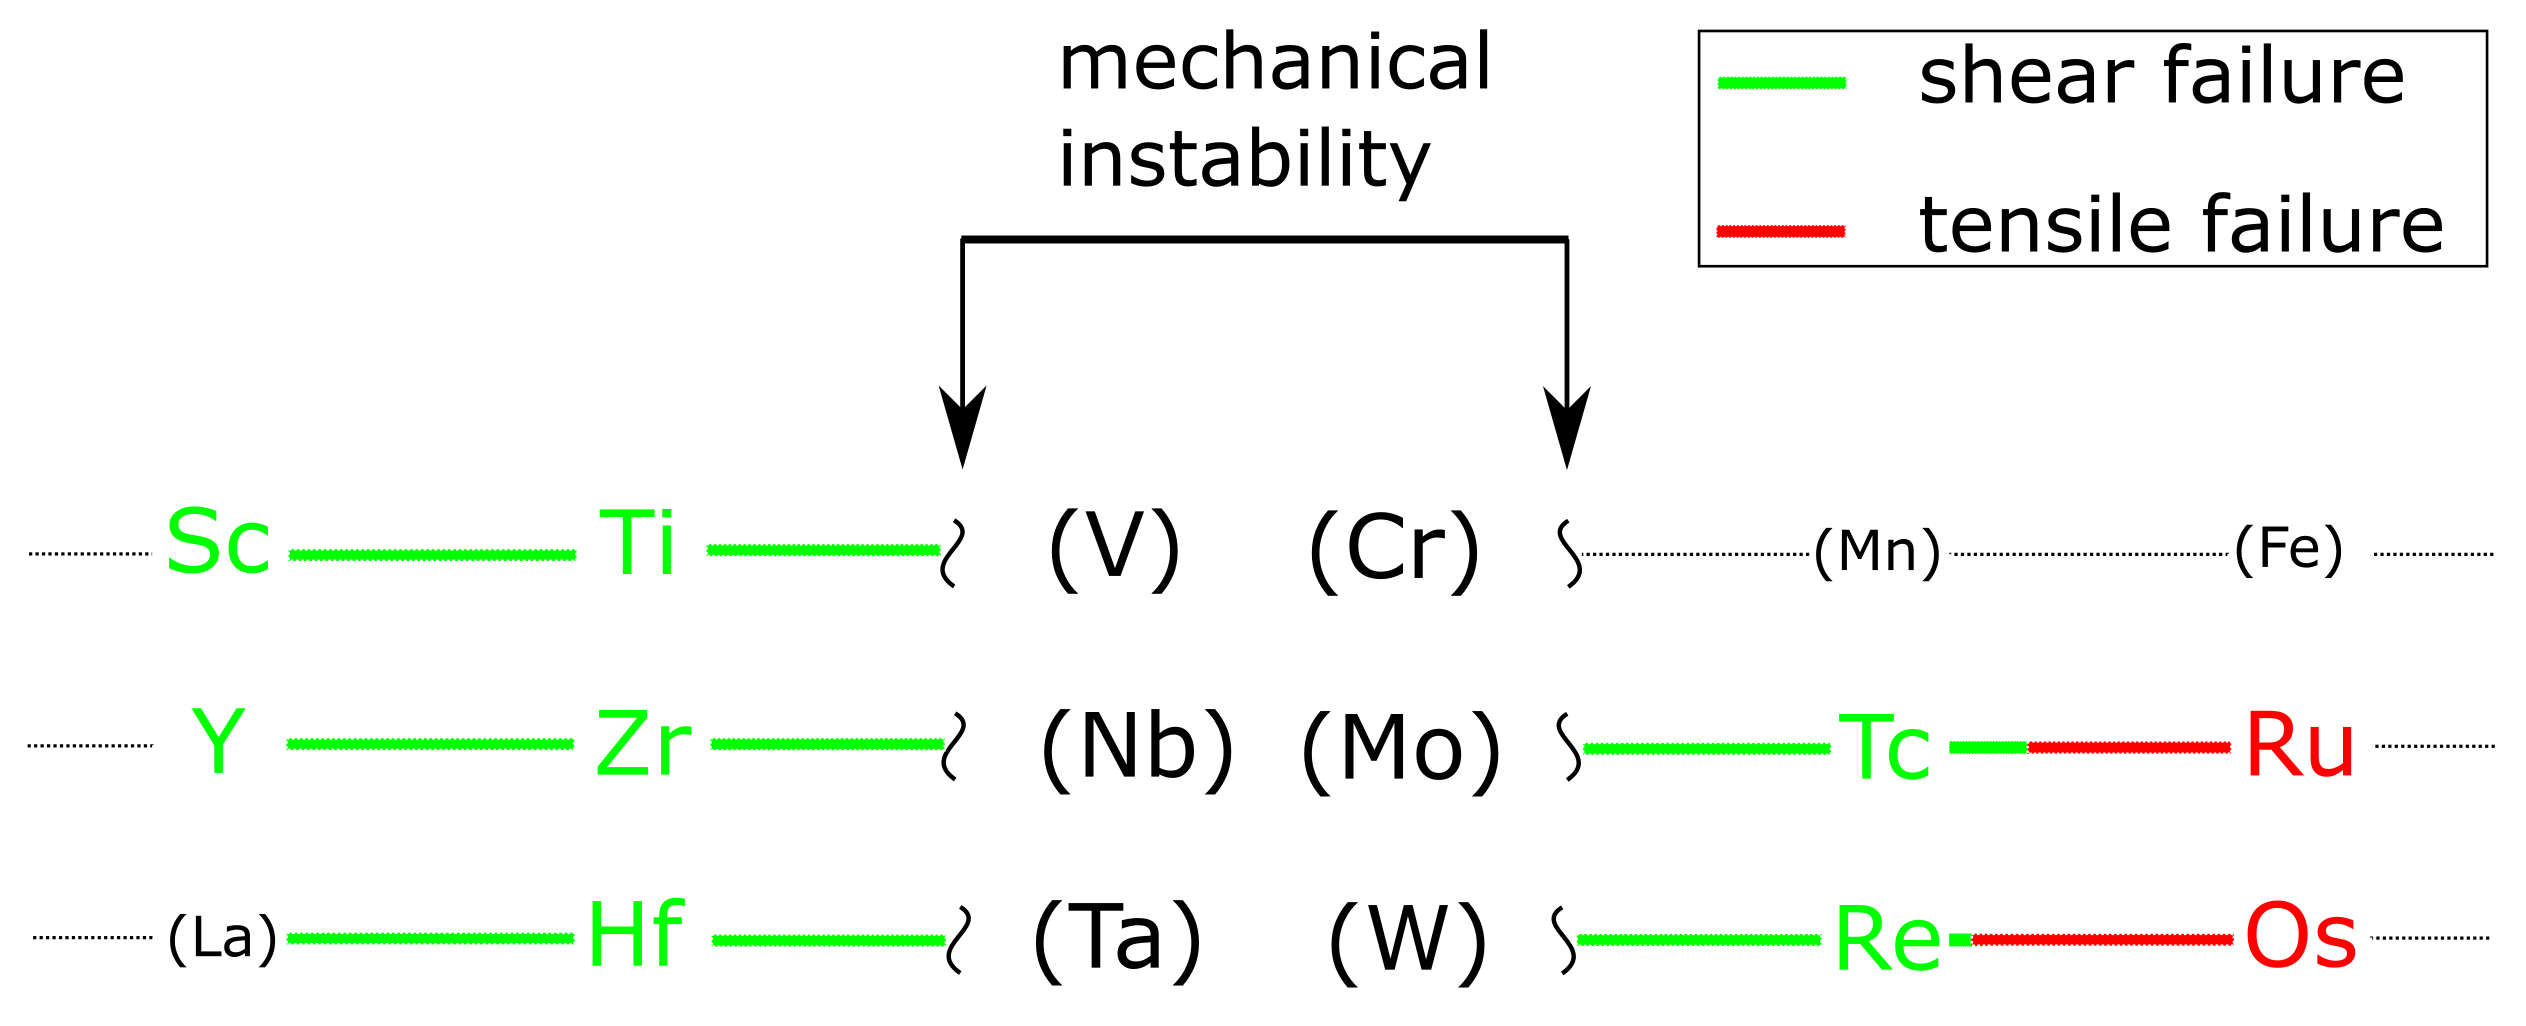
\includegraphics[width=0.50\textwidth]{drawing1.png}
\caption{Ideal failure mode-diagram vs. $d$-band filling in HCP metals and alloys}
\label{fig:sgentwinpic1}
\end{figure}

The formalism based on SOEC's and TOEC's developed in this work can be used to understand the physical grounds of shear vs. tensile failure. Consider first HCP materials with high shear moduli, $C_{44}$, such as Ru and Os. These metals are expected to exhibit high strength since that quantity scales with approximately the shear modulus. Such materials are therefore not likely to fail in shear, since the eigenvalue associated with shear failure (Eq. \ref{eqn:Wallace3}) is rather large and may not reach zero before the eigenvalue in Eq. \ref{eqn:Wallace4} does. Hence, this observation explains from an ideal strength point of view why strong materials tend to be brittle. Strong materials with a high shear modulus $C_{44}$ will only fail in shear and be accordingly intrinsically ductile according to Eq. \ref{eqn:Wallace3} if $\sigma_{33}$ is relatively large in magnitude, implying that $C_{33}$ is large. Further, the modulus $C_{333}$ is negative for most materials, implying softening of $C_{33}$ as the materials is strained along $c$ by $\xi$. A small magnitude of $C_{333}$ is also favorable for shear failure as it causes the magnitude of the stress $\sigma_{33}$ decrease less rapidly as a function of $\xi$. \\

Metals and alloys near half $d$-band filling such as Re and Tc are intrinsically ductile and fail in shear but are on the border of $d$-band filling regions where tensile failure occurs. Their shear failure is caused by an interplay of the SOEC's and TOEC's. First, the shear moduli $C_{44}$ of Re and Tc are large but smaller than those for Os and Ru. The same is true for the moduli $C_{33}$, but the ratio $C_{33}/C_{44}$ for group VII metals is larger than for group VIII metals, e.g. for Os  $C_{33}/C_{44} \approx 3.2$ whereas for Re $C_{33}/C_{44} \approx 4.5$. Second, for group VII metals and alloys, the magnitude of $C_{333}$ is smaller than for group VIII, which also promotes shear failure over tensile failure. Third, the TOEC $C_{344}$, which is a negative quantity for most materials, is relatively large in magnitude for group VII metals relative to those in group VIII. According to Eq. \ref{eqn:Cprime} (e), this implies that the shear modulus $C_{44}$ decreases relatively rapidly with strain $\xi$, which according to Eq. \ref{eqn:Wallace3}, favors a shear instability over a tensile instability.  \\

Finally, the high ductility HCP metals in group IV exhibit values of $C_{33}/C_{44}$ between approximately 4 and 6 which is higher than for groups VII and VIII. The relatively low values for $C_{44}$ cause the eigenvalue in Eq. \ref{eqn:Wallace3} to attain negative values before the eigenvalue in Eq. \ref{eqn:Wallace4}, and consequently to fail in shear.


\section{Conclusions}
In this work, the ideal deformation behavior and elastic stabilities of 14 HCP metals under uniaxial stress along the $c$-axis are studied: Be, Mg, Sc, Y, Ti, Zr, Hf, Tc, Re, Ru, Os, Co, Cd and Zn. It is found that out of these, 5 fail in tension along $c$ (Be, Mg, Ru, Os and Zn) whereas the 9 others fail in a shear mode. This leads to a natural division of the HCP-metals into 2 classes: intrinsically ductile or intrinsically brittle. Using a newly developed formalism, it is further shown that the critical strain and the deformation mode can be predicted from the SOEC's and TOEC's of the material. The formalism shows how the interplay between the SOEC's and TOEC's lead to a given failure mode and also indicated which particular elastic constants govern this process. It is found that HCP metals exhibiting high moduli $C_{44}$ are strong but for the same reason tend to fail in tension rather than shear and hence, are brittle. This occurs for transition metals and alloys in group VIII (Os, Ru). These materials also tend to have low values for $C_{33}/C_{44}$ and a lower Pugh ductility parameter $K/G$, where $K$ is the bulk modulus and $G$ the shear modulus \cite{pugh1954xcii}. The HCP metals in groups III and IV are found to be ductile, primarily due to their low shear moduli $C_{44}$ which promotes shear failure. The group VII HCP metals (Re, Tc) are an interesting case that combine a high shear modulus (strength) with intrinsically ductile behavior. The physical reason for this shear failure is the specific combination of SOEC's and TOEC's that this class of materials exhibits: a high $C_{33}$, but a relatively small magnitude of $C_{333}$ and a large magnitude of $C_{344}$. Finally, the trends of the ideal deformation behavior with $d$-band filling are revealed, resulting in approximate $d$-electron counts per atom for which an alloy is expected to fail in a ductile or brittle mode.


\bibliography{refs.bib}





\end{document} %EOPAPER



